\section{Questões}\label{sec:questoes}


\subsection{Questão 1}
Indique as etapas, como na Tabela 3.14, do algoritmo de busca direta à medida que ele monta o
banco de dados de roteamento para o nó A na rede mostrada na Figura 3.59.

\begin{figure}[H]
    \centering
    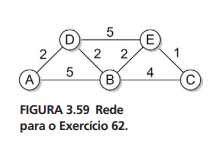
\includegraphics[width=0.7\textwidth]{images/ex_62.png}
    \caption{Rede mostrada na questão 1}
    \label{fig:questao_1}
\end{figure}

\begin{figure}[H]
    \centering
    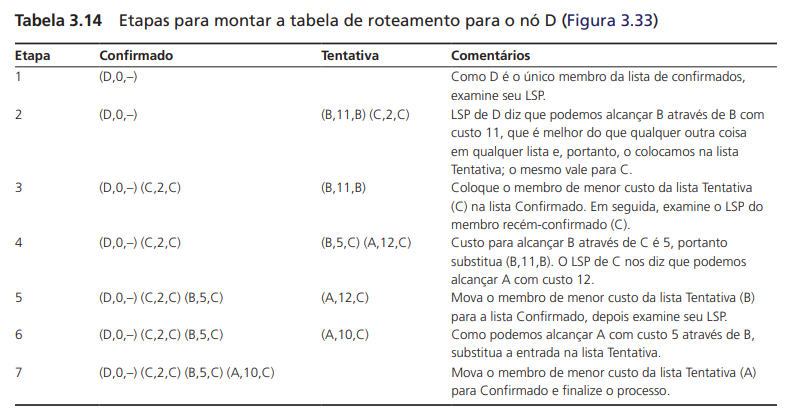
\includegraphics[width=0.9\textwidth]{images/tabela_3_14.png}
    \caption{Tabela 3.14 usada como referência para a questão} 
    \label{fig:questao_1_tabela}
\end{figure}

\subsection{Questão 2}
Suponha que um roteador tenha montado a tabela de roteamento mostrada na Tabela 3.18. O
roteador pode entregar pacotes diretamente pelas interfaces 0 e 1, ou então pode encaminhar
pacotes aos roteadores R2, R3 ou R4. Descreva o que o roteador faz com um pacote endereçado a
cada um dos seguintes destinos:

\begin{enumerate}[label=\alph*.]
    \item 128.96.39.10
    \item 128.96.40.12
    \item 128.96.40.151
    \item 192.4.153.17
    \item 192.4.153.90
\end{enumerate}

\begin{figure}[H]
    \centering
    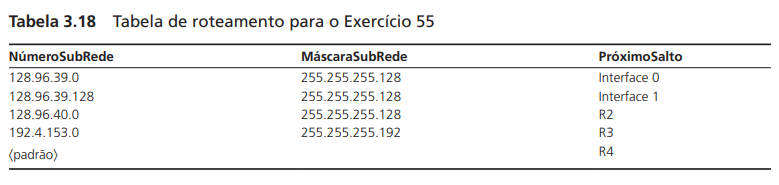
\includegraphics[width=0.8\textwidth]{images/tabela_3_18.png}
    \caption{Tabela 3.18 usada como referência para a questão} 
    \label{fig:questao_2_tabela}
\end{figure}

\subsection{Questão 3}
A Tabela 3.20 é uma tabela de roteamento usando CIDR. Os bytes de endereço estão em
hexadecimal. A notação “/12” em C4.50.0.0/12 indica uma máscara de rede com 12 bits 1 iniciais:
FF.F0.0.0. Observe que as três últimas entradas abrangem cada endereço e, portanto, podem ser usadas no lugar de uma rota padrão. 
Indique para qual próximo salto os pacotes com os seguintes endereços serão entregues:

\begin{enumerate}[label=\alph*.]
    \item C4.5E.13.87
    \item C4.5E.22.09
    \item C3.41.80.02
    \item 5E.43.91.12
    \item C4.6D.31.2E
    \item C4.6B.31.2E
\end{enumerate}

\begin{figure}[H]
    \centering
    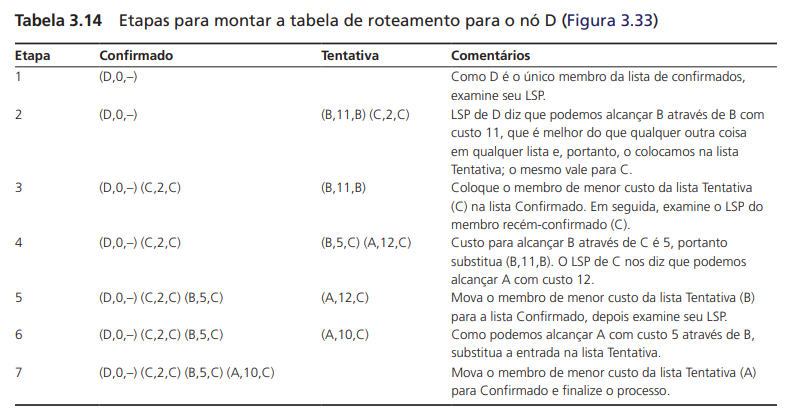
\includegraphics[width=0.8\textwidth]{images/tabela_3_14.png}
    \caption{Tabela 3.20 usada como referência para a questão} 
    \label{fig:questao_3_tabela}
\end{figure}

\subsection{Questão 4}
Leiam a Seção 4.2 do livro-texto (exceto os trechos sobre “Multicast
interdomínios - MSDP” e “Árvores bidirecionais - BIDIR-PIM”) e respondam:

\begin{enumerate}[label=\alph*.]
    \item Além da entrega de pacotes aos destinos, qual é a principal preocupação de um
    protocolo de roteamento multicast?
    \item Qual é o papel do IGMP no esquema de funcionamento multicast do IP?
    \item Compare brevemente as estratégias DVMRP e PIM-SM, mostrando as vantagens e
    desvantagens de cada uma.
    \item Que características adicionais o PIM-SSM traz em relação ao PIM-SM?
\end{enumerate}